\section{Experiments and Results}\label{sec:experiments}
After presenting the separation constraints, we test our formulation in a series of experiments to test our rationale and create insights from our proposal. Purposely, we chose three datsets in our experimentation: the \moons dataset (sampling $100$ points, $85$ for training and $15$ for validation), the \texttt{MNIST} dataset as described in LeCun and Cortes. \cite{mnist} and the \texttt{CIFAR-10} dataset devised by Krizhevsky and described in \cite{cifar10}.
\\\\
Inspired by Hasanpour et al. in \cite{simpnet}, we investigate the effect of the constraint formulation on different choices of depth and width, training a family of \emph{rectangular} networks (i.e. networks with fixed layer width $m_k=W$ as presented in our layer function formulation on Equation \ref{eq:layer}) as shown in Table \ref{tab:grids}.
\\\\

\begin{table}[]
\centering
\begin{tabular}{@{}lll@{}}
\toprule
         & Depth & Width \\ \midrule
Moons    & 1-150 & 1-25  \\
MNIST    & 2-64  & 2-8   \\
CIFAR-10 & 1-40  & 10    \\ \bottomrule
\end{tabular}
\caption{}\label{tab:grids}
\end{table}

All the networks used were optimized using Adam \cite{adam}. More specifically, for the \moons dataset we used a learning rate of $0.01$ for $10000$ epochs and a batch size of $85$. Meanwhile, for both \texttt{MNIST} and \texttt{CIFAR-10} we used a learning rate of $0.0001$ for $50$ epochs and a batch size of $1024$. We used an Glorot uniform initialization scheme \cite{Glorot10Initialization} (by default on \texttt{Keras}). We used $\lambda_{MOONS}=10^-4$ $\lambda_{MNIST}=\lambda_{CIFAR}=10^{-8}$ for the Separation Constraints. Our experiments were conducted using \texttt{Keras} \cite{keras} and \texttt{TensorFlow} \cite{tensorflow}, fixing the random seed to an arbitrary value of $10$. 
\\\\
Our findings are based on a comparison of our proposal to feed-fordward \ReLU networks \cite{relu} and Batch Normalization as described in \cite{batchnorm}. More specifically, we compare them against three different versions of the Separating Constraints: unit-based \SepUnit (see Subsection \ref{subsec:sepUnit}), point-based \SepPoint (see Subsection \ref{subsec:sepPoint}) and the combination of both that we denote by \SepUnitPoint.
\\\\

% WIDTH VS DEPTH STARTS HERE
Figure \ref{fig:moons_grid} shows how training deeper networks requires an increment on the layer width, as stated by Hasanpour et al. \cite{simpnet} or Huang et al. \cite{densenet}. This is suggested by beige colored region in \ref{fig:moons_grid_relubn} for \ReLUBN. Particularly, we advocate that for each depth $D$, there exists a particular width $W_{min}$, for which maximal accuracy is obtained at depth $D$. We propose the following definition for $W_{min}$:
\begin{equation}\label{eq:dependencyWidthDepth}
 W_{min}(D) = 
 \begin{cases}
 \hat{W}_{min}, & D\leq \hat{D}\\
 \hat{W}_{min}+\max\{0,h(D)-\hat{D}\}, & D\leq \hat{D}\\
 \end{cases}
\end{equation}
for $h:\mathbb{R}\rightarrow\mathbb{R}$ a non-negative, monotonically increasing function such that $h(0)\geq 0$. 
Here, we suggest that $\hat{D}$ is the depth at which the width-increase starts being required. In this sense, $\hat{W}_{min}$ can be understood as the minimum width for which maximal accuracy can be obtained. 
\\\\
In this sense, for $D\geq \hat{D}$, $\Delta{W} = W-W_{min}(D)$ quantifies the number of additional units per-layer that do not contribute in matters of accuracy formation: they are devoted to find a combination of hyper-planes to \emph{enable} back-propagation. On the one hand, this is interpretable in terms of the sets defined on section \ref{sec:separability} (i.e. $\Delta{W}$ additional units that ensure that $I(\layer)\neq\emptyset$), on the other we suggest that larger values of $\hat{D}$ delay the need for the width-increase strategy. In addition, we claim that $\hat{W}_{min}$ is \emph{dataset dependent}, whereas $\hat{D}$ is related with its well-posedness of the architecture of the network with regards to back-propagation.
\\\\
Experimentally, we observe that by using \SepUnitPoint the value of $\hat{D}$ is more than doubled than by using \ReLUBN ($40$ vs $15$, as Table \ref{tab:dependency}). In this sense, our claim  that separation constraints enables to train deeper networks with the same width, is verified (as showcased by Figures \ref{fig:moons_grid_u}, \ref{fig:moons_grid_p} and \ref{fig:moons_grid_up}). We provide the reader with Table \ref{tab:dependency} to summarize our findings with regards to $\hat{D}$ and $W_{min}$ in the scope of our experimentation. 
\\\\

\begin{table}[]
\begin{tabular}{@{}lll@{}}
\toprule
        & $\hat{W_{min}}$ & $\hat{D}$ \\ \midrule
\ReLU   & 3         & 4             \\
\ReLUBN & 3         & 15            \\
\SepUnit   & 2-3       & 10            \\
\SepPoint   & 3-4       & 45            \\
\SepUnitPoint  & 2-3       & 40            \\ \bottomrule
\end{tabular}
\caption{Summary of minimum widths and depths related to maximal accuracy obtained comparing \ReLUBN and the different versions of \SepConstraint, trained using the \moons dataset, a learning rate of $0.01$ and $\lambda = 0.0001$ for all \SepConstraint variants.}\label{tab:dependency}
\end{table}
When observing the differences between variants of \SepConstraint we observe that \SepUnit follows a pattern similar to \ReLUBN, but avoids failures (see the lack of black boxes in Figure \ref{fig:moons_grid_u} in contrast to Figure \ref{fig:moons_grid_relubn}, particularly when $D\geq 15$).  
\\\\
Meanwhile, \SepPoint (Figure \ref{fig:moons_grid_p}) possesses a larger value of $\hat{D}$  than both \ReLUBN and \SepUnit (see second column of Table \ref{tab:dependency}). However, it suffers from the same abrupt breakdown as \ReLU but with an small successful area within the values of $W=5$ and $W=10$ and $D\geq 100$. 
\\\\
Finally, integrating \SepUnit and \SepPoint to use \SepUnitPoint (Figure \ref{fig:moons_grid_up}) improves both accuracy, minimizes the value of $W_{min}$ (to the level of\SepUnit) and goes in terms of $\hat{D}$ beyond \SepPoint. Suggesting that unit-based separation and point-based separation is mutually beneficial.
\\\\
The constraint formulation also proves beneficial when on convolutional networks, as tested using other popular datasets (in our case \texttt{MNIST} and \texttt{CIFAR-10}). As Figure \ref{fig:mnist_grid} shows a similar behaviour to the \moons dataset (Figure\ref{fig:moons_grid}): \ReLU breaks down after few layers, \ReLUBN  delays the degradation of accuracy (has a larger $\hat{D}$ value), while \SepUnitPoint remains functional regardless of $D$. 
\\\\
Similarly, our experiments with the \texttt{CIFAR-10} dataset (as presented on Table \ref{tab:cifar10}) behaves a little bit differently. Though the same accuracy degradation observed for \moons and \texttt{MNIST} while \SepUnitPoint allows for a larger value of $\hat{D}$, accuracies reached are not dramatically improved by the introduction of separation constraints. However, it is during the validation phase, that \SepConstraint maintains accuracy levels, while \ReLUBN degrades. However, we blame these decreased accuracy levels to a limited choice of $W$ inferior to $\hat{W}_{min}$.  

\begin{figure*}
  \centering
    \begin{subfigure}[b]{0.3\textwidth}
        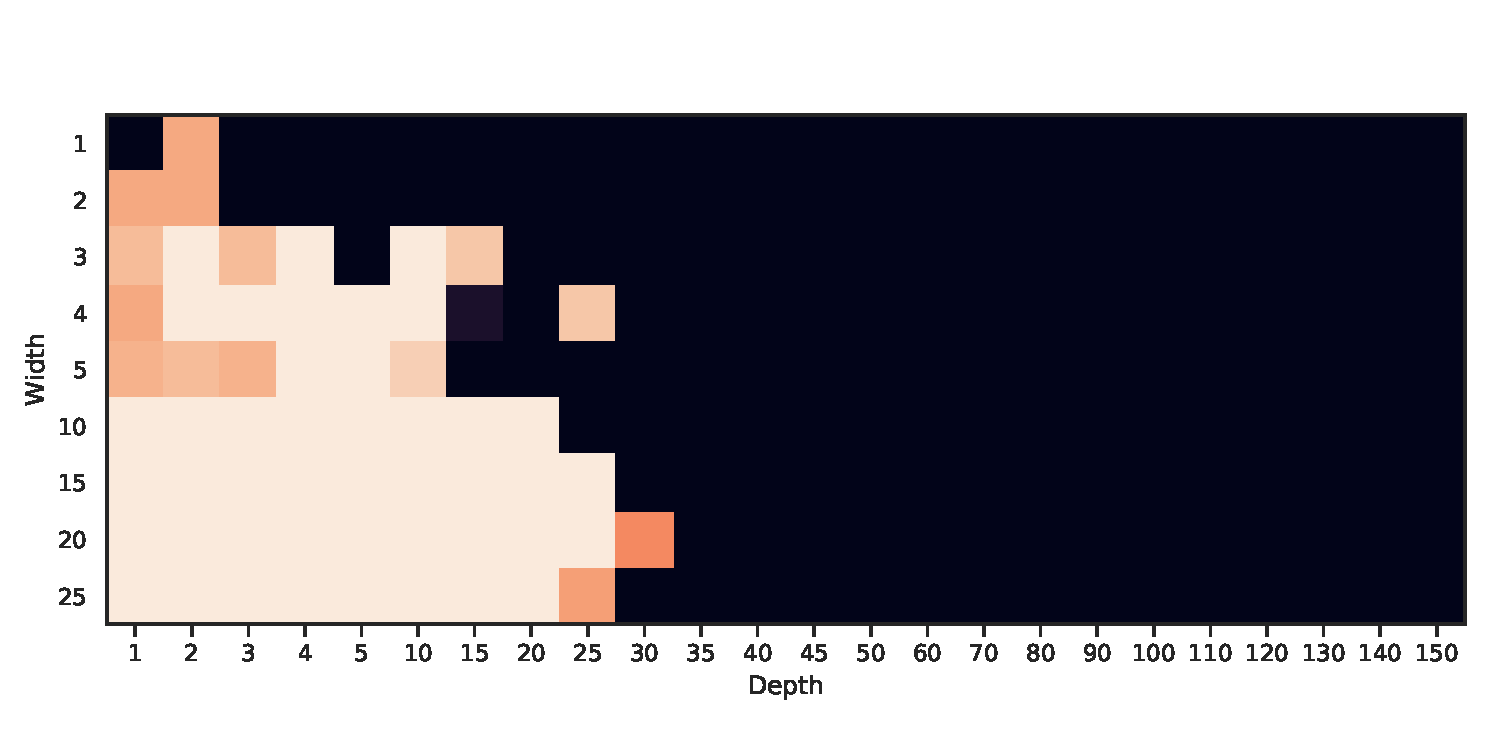
\includegraphics[width=\textwidth]{img/moons_grid/acc-relu.pdf}
        \caption{\ReLU training}
        \label{fig:moons_grid_relu}
    \end{subfigure}
    ~ %add desired spacing between images, e. g. ~, \quad, \qquad, \hfill etc. 
      %(or a blank line to force the subfigure onto a new line)
    \centering
    \begin{subfigure}[b]{0.3\textwidth}
        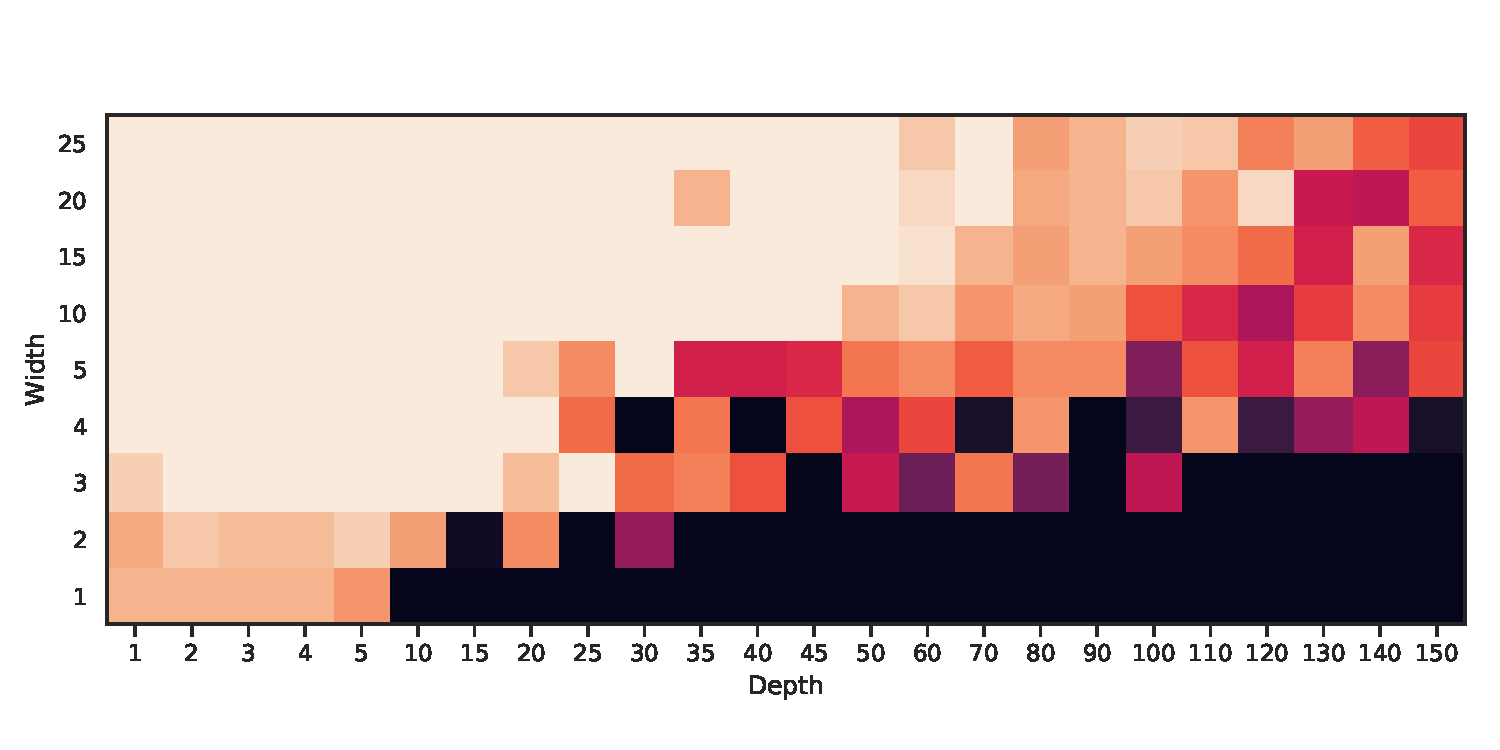
\includegraphics[width=\textwidth]{img/moons_grid/acc-relu-bn.pdf}
        \caption{\ReLUBN training}
        \label{fig:moons_grid_relubn}
    \end{subfigure}
    ~ %add desired spacing between images, e. g. ~, \quad, \qquad, \hfill etc. 
      %(or a blank line to force the subfigure onto a new line)
    \centering
    \begin{subfigure}[b]{0.3\textwidth}
        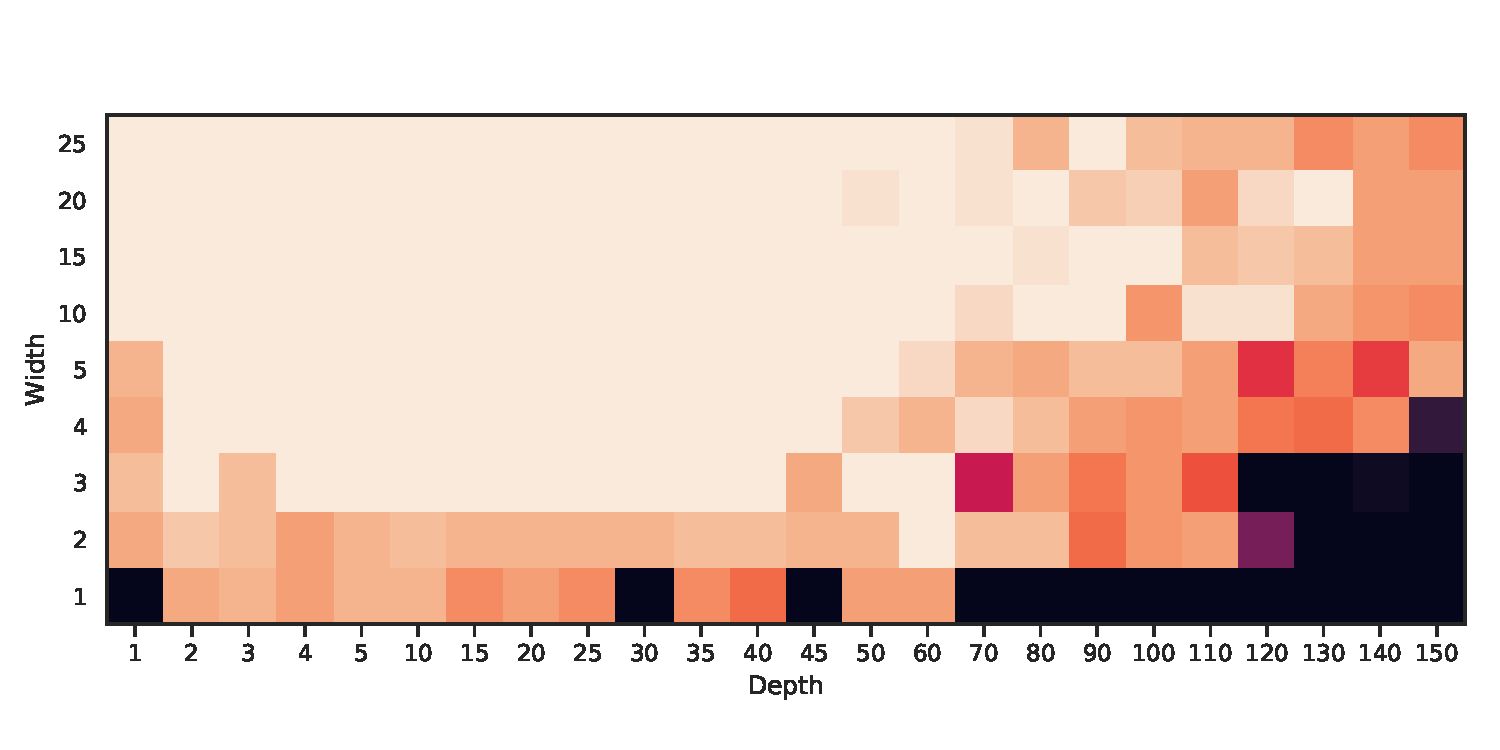
\includegraphics[width=\textwidth]{img/moons_grid/acc-sep-up-0-0001.pdf}
        \caption{\SepUnitPoint training}
        \label{fig:moons_grid_up}
    \end{subfigure}
    ~ %add desired spacing between images, e. g. ~, \quad, \qquad, \hfill etc. 
      %(or a blank line to force the subfigure onto a new line)
    \\
    \begin{subfigure}[b]{0.3\textwidth}
        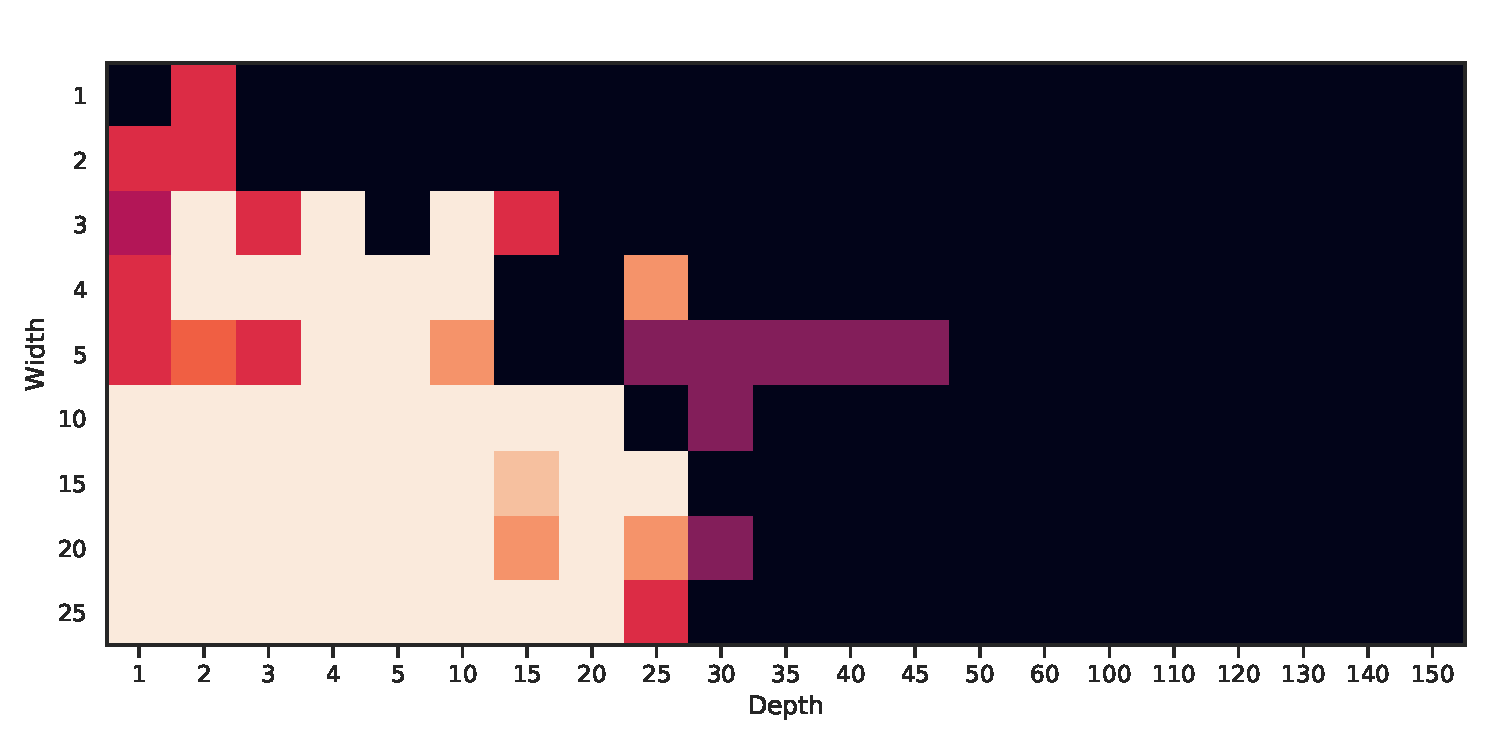
\includegraphics[width=\textwidth]{img/moons_grid/val-acc-relu.pdf}
        \caption{\ReLU validation}
        \label{fig:moons_grid_relu}
    \end{subfigure}
    ~ %add desired spacing between images, e. g. ~, \quad, \qquad, \hfill etc. 
      %(or a blank line to force the subfigure onto a new line)
    \centering
    \begin{subfigure}[b]{0.3\textwidth}
        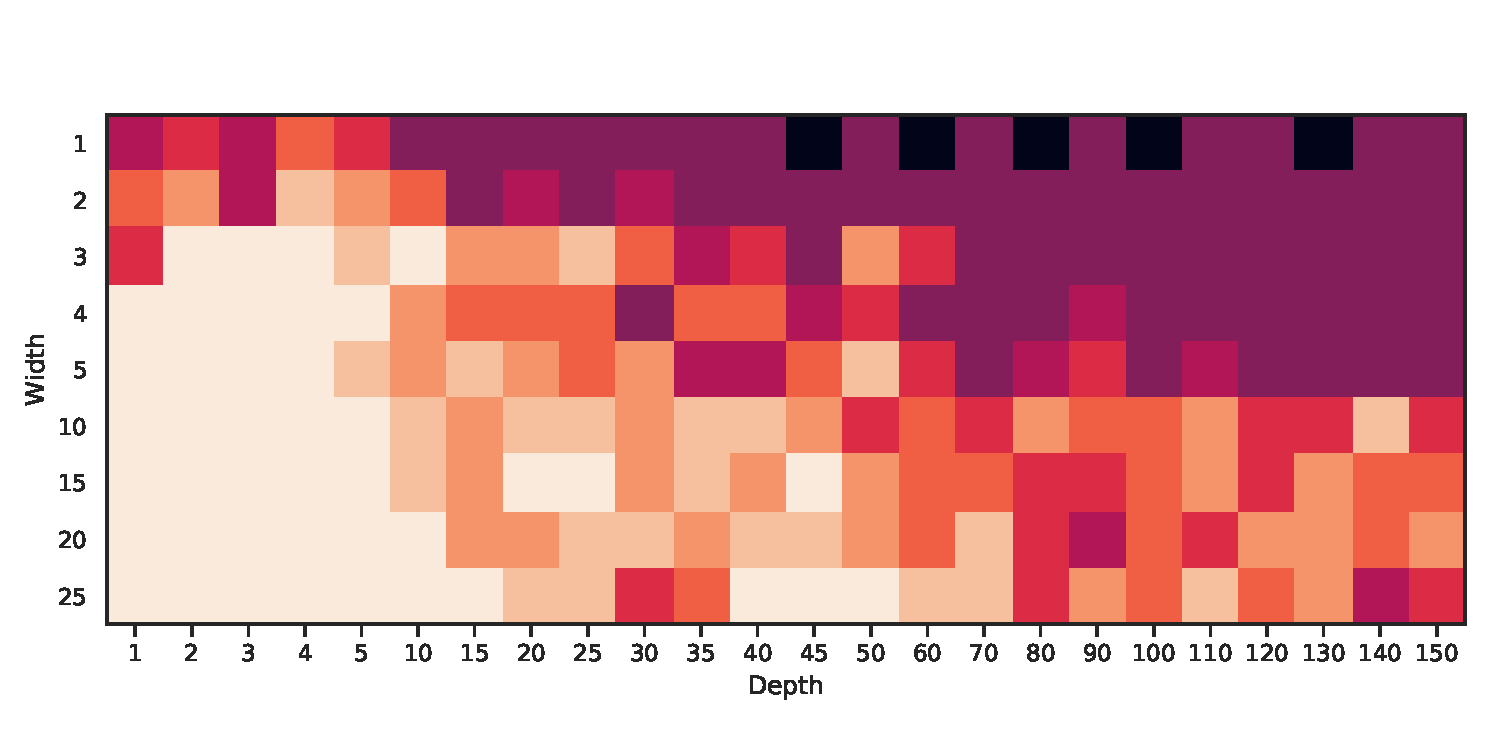
\includegraphics[width=\textwidth]{img/moons_grid/val-acc-relu-bn.pdf}
        \caption{\ReLUBN validation}
        \label{fig:moons_grid_relubn}
    \end{subfigure}
    ~ %add desired spacing between images, e. g. ~, \quad, \qquad, \hfill etc. 
      %(or a blank line to force the subfigure onto a new line)
    \centering
    \begin{subfigure}[b]{0.3\textwidth}
        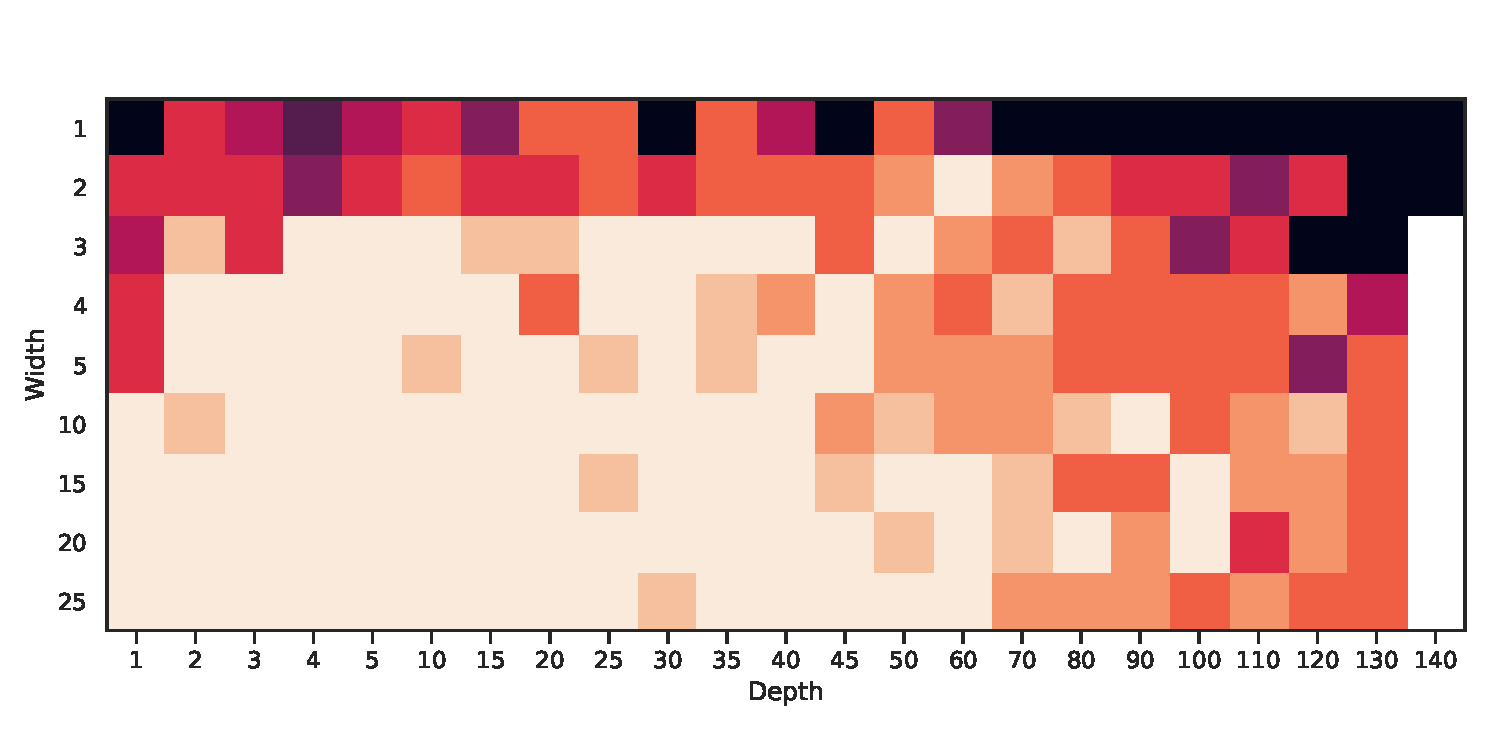
\includegraphics[width=\textwidth]{img/moons_grid/val-acc-sep-up-0-0001.pdf}
        \caption{\SepUnitPoint validation}
        \label{fig:moons_grid_up}
    \end{subfigure}
    ~ %add desired spacing between images, e. g. ~, \quad, \qquad, \hfill etc. 
      %(or a blank line to force the subfigure onto a new line)
      \\
    \begin{subfigure}[b]{0.3\textwidth}
        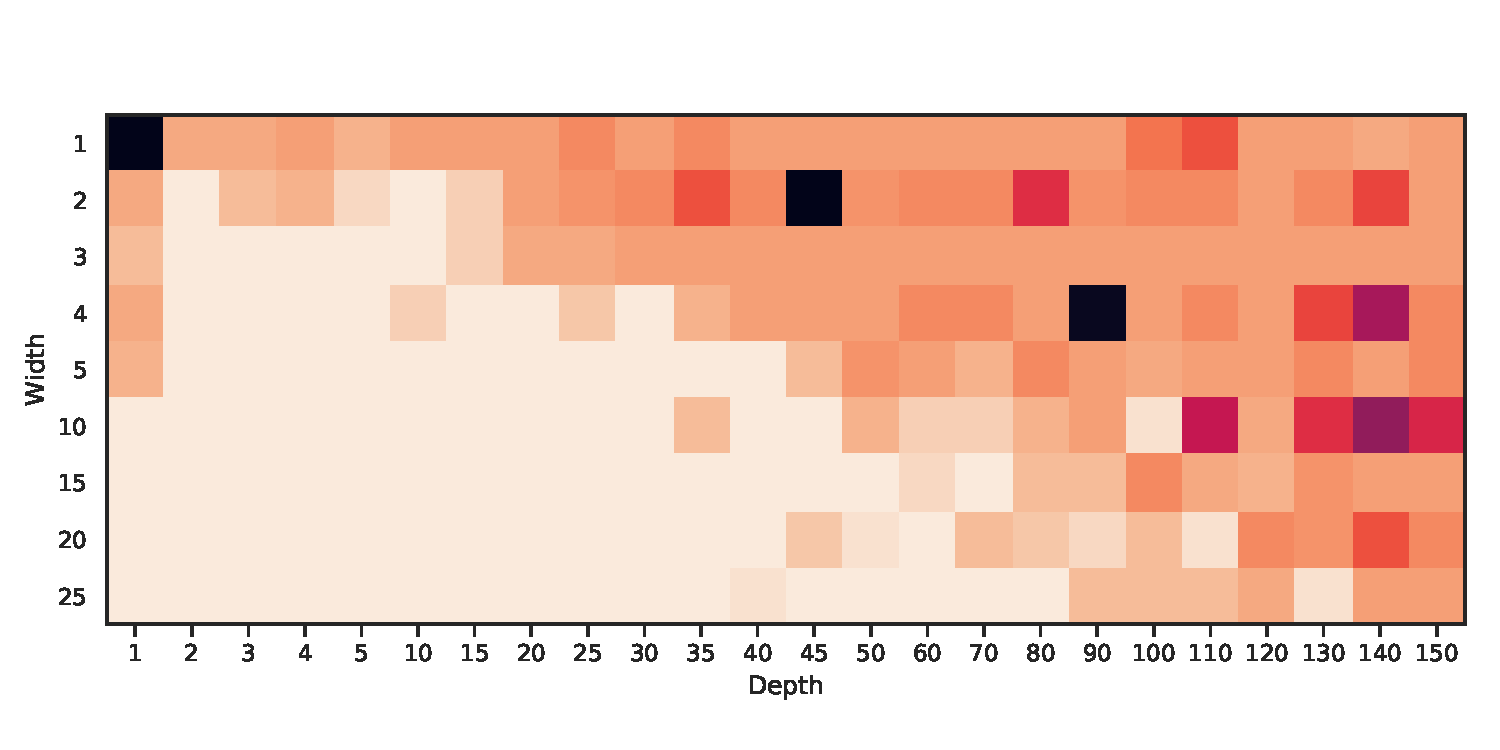
\includegraphics[width=\textwidth]{img/moons_grid/acc-sep-u-0-0001.pdf}
        \caption{\SepUnit training}
        \label{fig:moons_grid_u}
    \end{subfigure}
    ~ %add desired spacing between images, e. g. ~, \quad, \qquad, \hfill etc. 
      %(or a blank line to force the subfigure onto a new line)
    \centering
    \begin{subfigure}[b]{0.3\textwidth}
        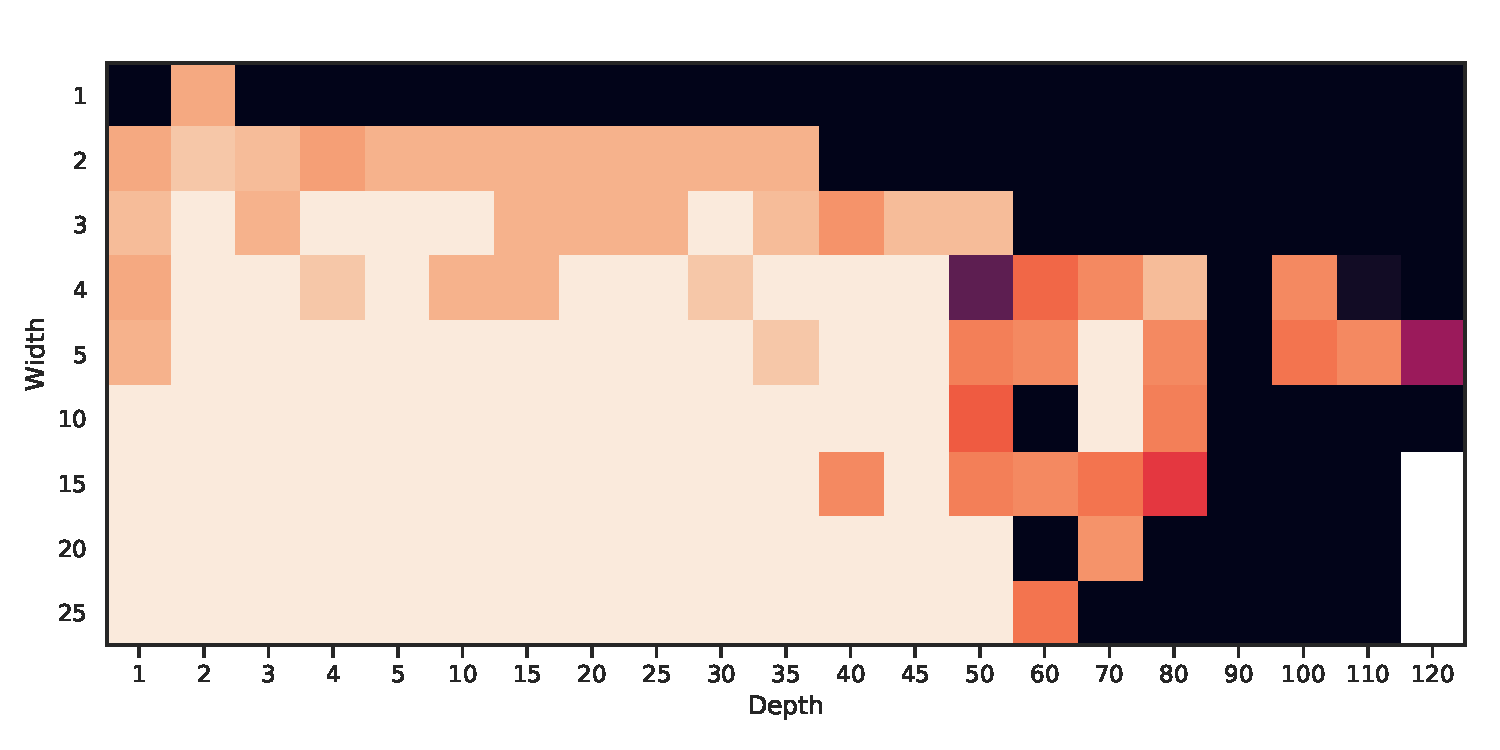
\includegraphics[width=\textwidth]{img/moons_grid/acc-sep-p-0-0001.pdf}
        \caption{\SepPoint training}
        \label{fig:moons_grid_p}
    \end{subfigure}
    ~ %add desired spacing between images, e. g. ~, \quad, \qquad, \hfill etc. 
      %(or a blank line to force the subfigure onto a new line)
    \\
    \begin{subfigure}[b]{0.3\textwidth}
        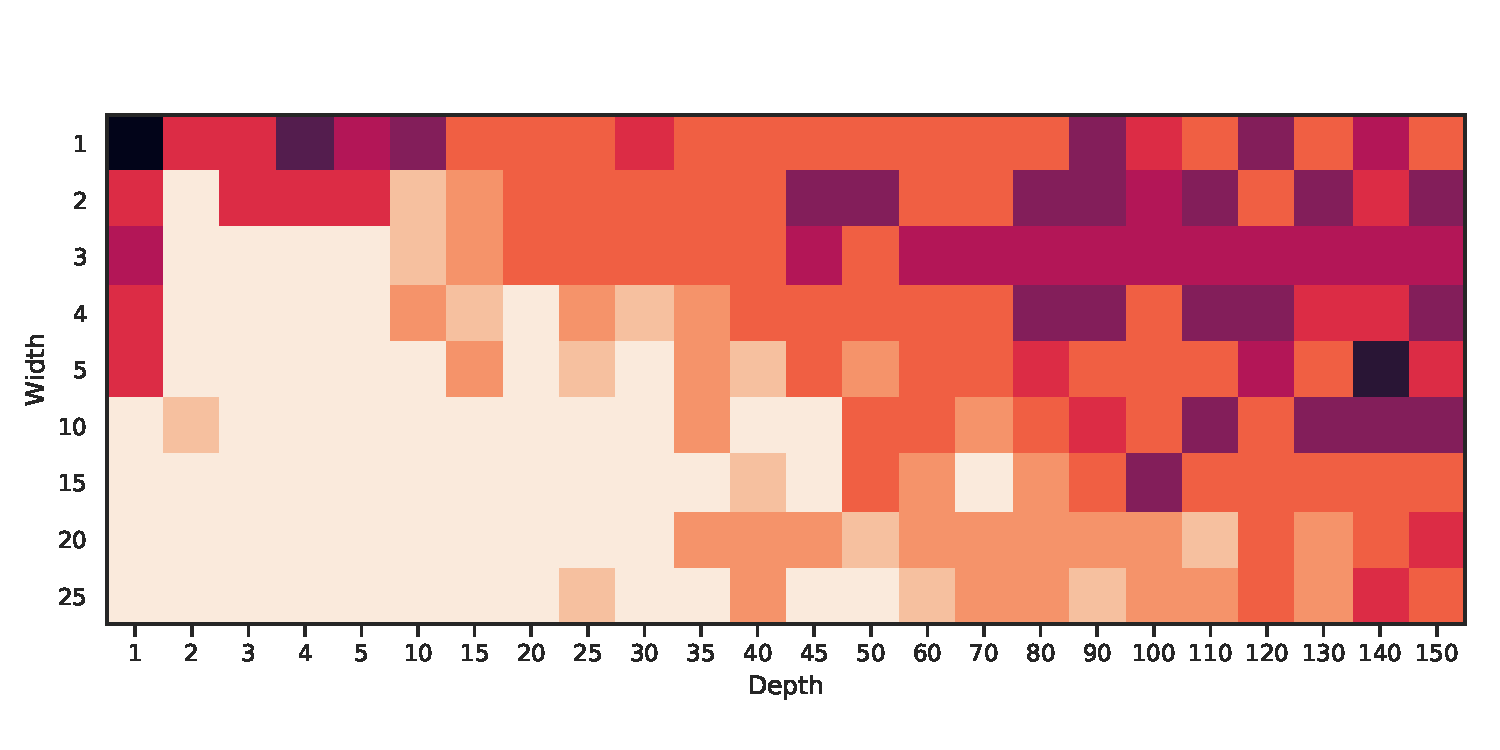
\includegraphics[width=\textwidth]{img/moons_grid/val-acc-sep-u-0-0001.pdf}
        \caption{\SepUnit validation}
        \label{fig:moons_grid_u}
    \end{subfigure}
    ~ %add desired spacing between images, e. g. ~, \quad, \qquad, \hfill etc. 
      %(or a blank line to force the subfigure onto a new line)
    \centering
    \begin{subfigure}[b]{0.3\textwidth}
        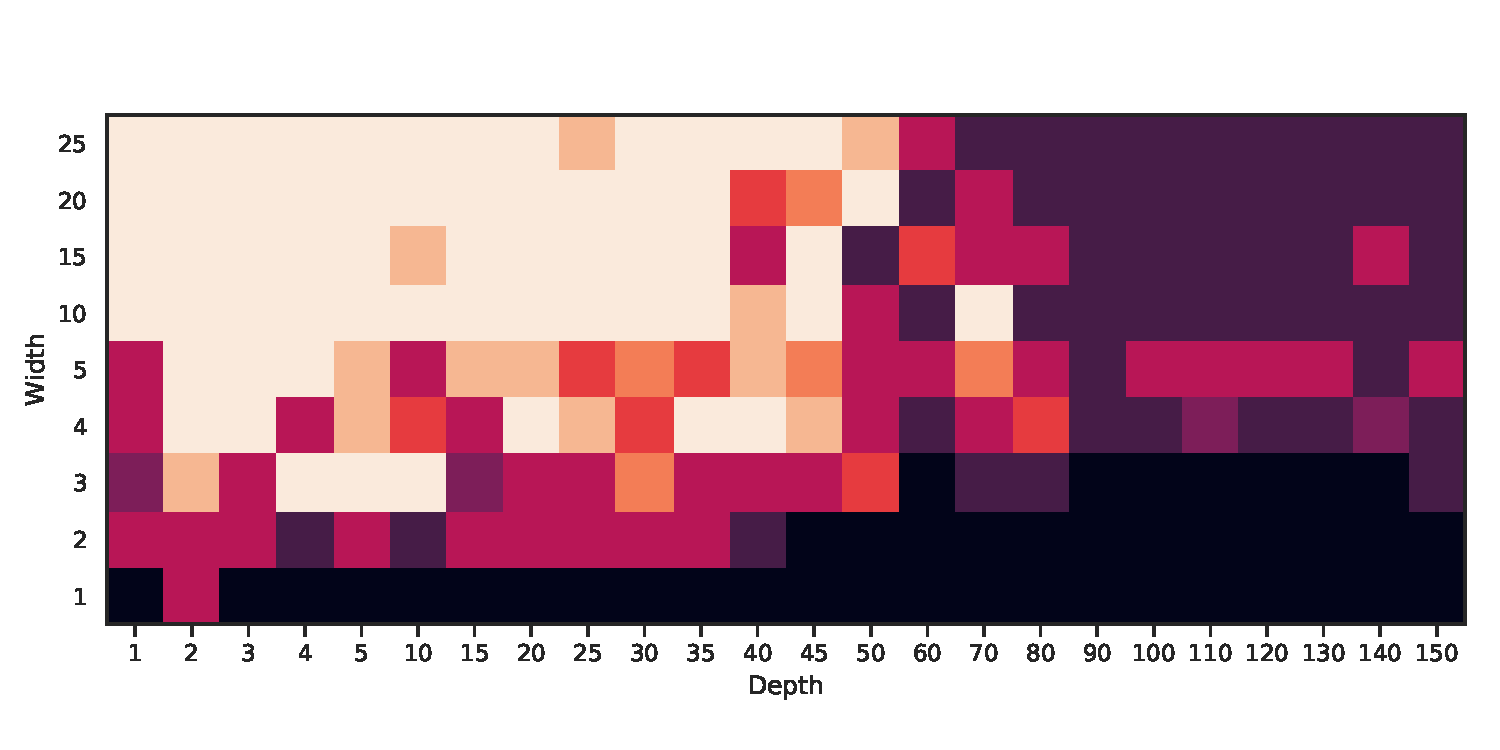
\includegraphics[width=\textwidth]{img/moons_grid/val-acc-sep-p-0-0001.pdf}
        \caption{\SepPoint validation}
        \label{fig:moons_grid_p}
    \end{subfigure}
    ~ %add desired spacing between images, e. g. ~, \quad, \qquad, \hfill etc. 
      %(or a blank line to force the subfigure onto a new line)
    
    
  \caption{Depth vs Width accuracy plot a for rectangular network using a grid (width from $2$ to $25$ and depth from $2$ to $150$),  trained using a Adam learning rate of $0.01$ in the \moons dataset. The color show the accuracy attained of each of the combinations of width and depth, the clearer the better. Notice how \ReLU, Figure \ref{fig:moons_grid_relu}, fails with networks deeper than 30 layers. In other hand, \ReLUBN, Figure \ref{fig:moons_grid_relubn}, manages to work until 70 layers deep. \SepUnitPoint,  Figure \ref{fig:moons_grid_up}, works significantly better than both, up to 120 layers. Notice how all the methods suffer from degradation from depth, which is partially alleviated by the use of greater width. This is consistent with \cite{simpnet} and \cite{densenet}. However, \SepUnitPoint is able to delay the apparition of the issue. This is especially visible when the number of units is small (from $2$ to $5$) where \ReLUBN fails to work whereas \SepUnitPoint does not. Regarding to the role of the constraint on its success, we find that \SepUnit, Figure \ref{fig:moons_grid_u}, allows the network to grow deeper, yet the accuracy can be lower following the linear decrease with the inverse of the width, which we blame on the inability of the \SepUnit constraint to address the \emph{dead point} issue. In the other hand, \SepPoint, Figure \ref{fig:moons_grid_p}, seems to perform well up to 50 layers, but it breaks down afterwards. Finally, \SepLayer , Figure \ref{fig:moons_grid_l} seems to suffer if the width is too large, performing well up to 70 layers.}
  \label{fig:moons_grid} 
\end{figure*}


\begin{figure*}
  \centering
    \begin{subfigure}[b]{0.3\textwidth}
        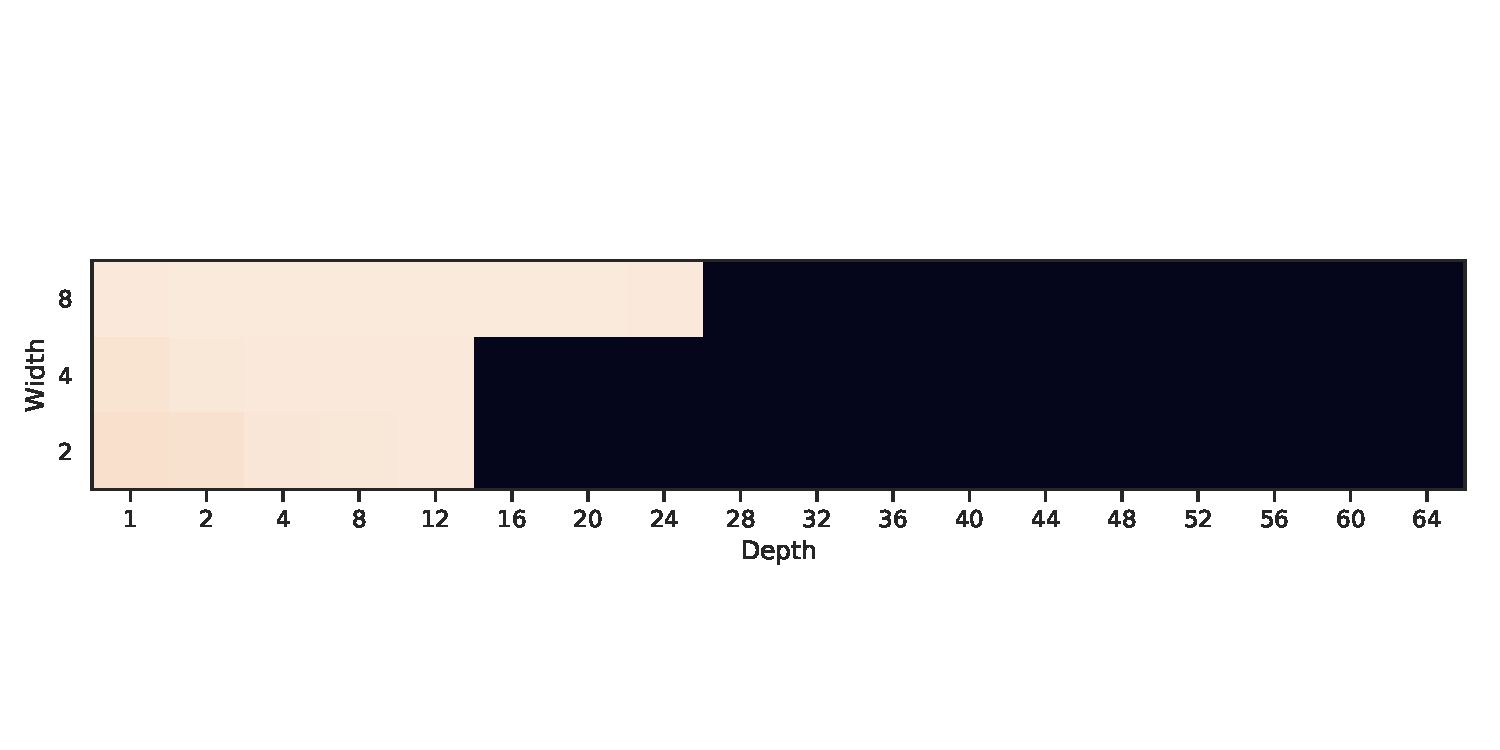
\includegraphics[width=\textwidth]{img/mnist_grid/acc-relu-ks-3x3-bs-1024.pdf}
        \caption{\ReLU}
        \label{fig:mnist_grid_relu}
    \end{subfigure}
    ~ %add desired spacing between images, e. g. ~, \quad, \qquad, \hfill etc. 
      %(or a blank line to force the subfigure onto a new line)
    \centering
    \begin{subfigure}[b]{0.3\textwidth}
        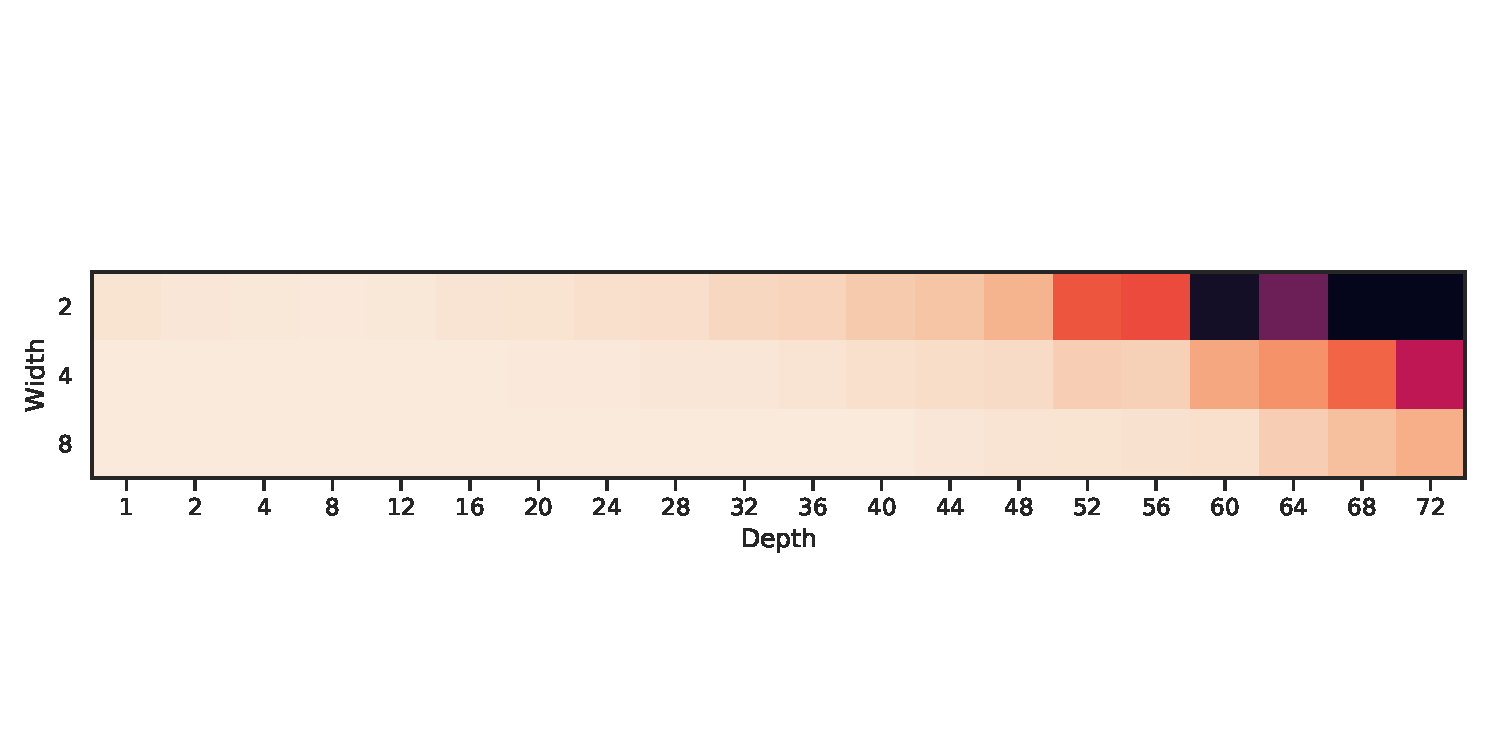
\includegraphics[width=\textwidth]{img/mnist_grid/acc-relu-bn-ks-3x3-bs-1024.pdf}
        \caption{\ReLUBN}
        \label{fig:mnist_grid_relubn}
    \end{subfigure}
    ~ %add desired spacing between images, e. g. ~, \quad, \qquad, \hfill etc. 
      %(or a blank line to force the subfigure onto a new line)
    \centering
    \begin{subfigure}[b]{0.3\textwidth}
        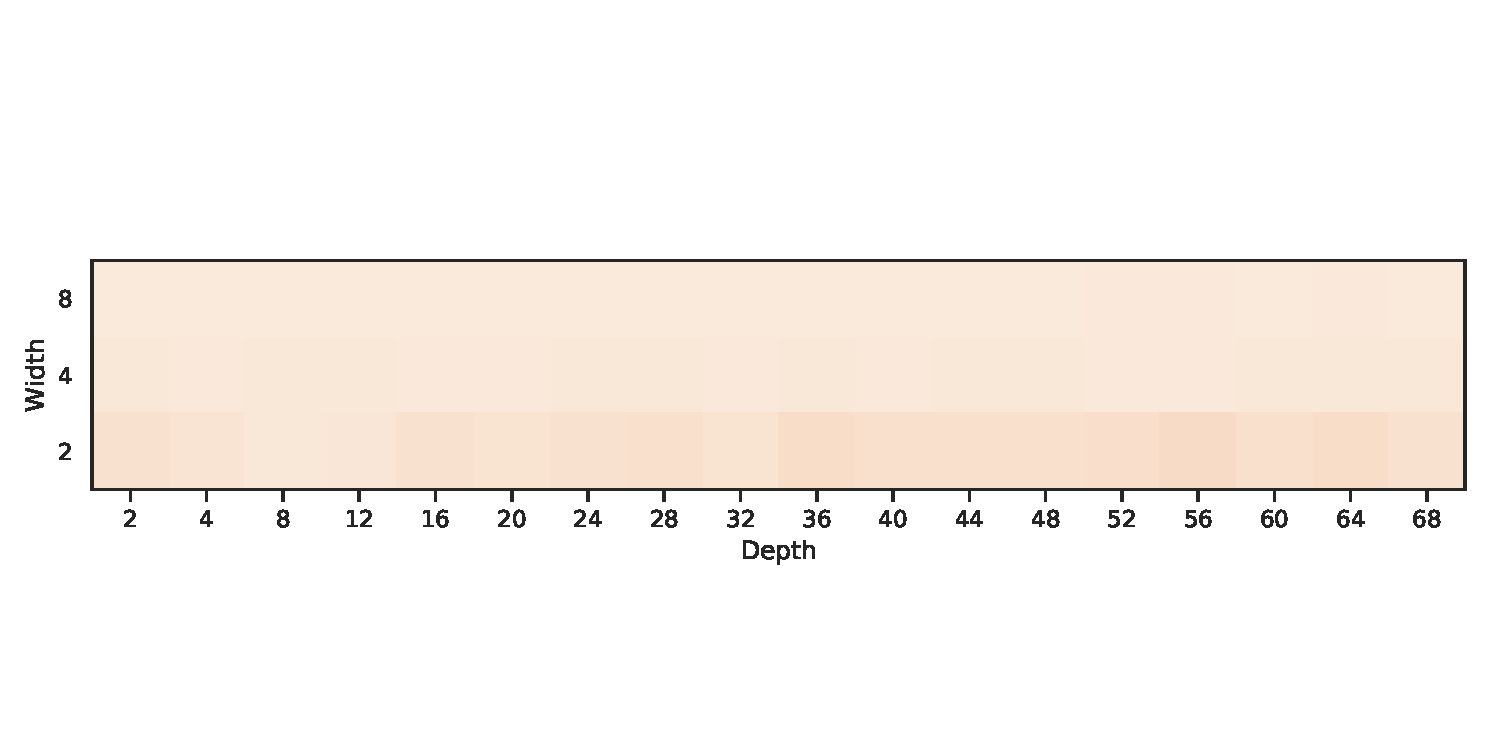
\includegraphics[width=\textwidth]{img/mnist_grid/acc-sep-up-1e-08-ks-3x3-bs-1024.pdf}
        \caption{\SepUnitPoint}
        \label{fig:mnist_grid_up}
    \end{subfigure}
    ~ %add desired spacing between images, e. g. ~, \quad, \qquad, \hfill etc. 
      %(or a blank line to force the subfigure onto a new line)
    
  \caption{Depth vs Width accuracy plot a for rectangular network using a grid (width from $2$ to $25$ and depth from $2$ to $150$),  trained using a Adam learning rate of $0.01$ in the MNIST dataset. The color show the accuracy attained of each of the combinations of width and depth, the clearer the better. Notice how \ReLU, Figure \ref{fig:mnist_grid_relu}, fails with networks deeper than 30 layers. In other hand, \ReLUBN, Figure \ref{fig:mnist_grid_relubn}, manages to work until 70 layers deep. \SepUnitPoint,  Figure \ref{fig:mnist_grid_up}, works significantly better than both, up to 120 layers. Notice how all the methods suffer from degradation from depth, which is partially alleviated by the use of greater width. This is consistent with \cite{simpnet} and \cite{densenet}. However, \SepUnitPoint is able to delay the apparition of the issue. This is especially visible when the number of units is small (from $2$ to $5$) where \ReLUBN fails to work whereas \SepUnitPoint does not.}
  \label{fig:mnist_grid} 
\end{figure*}


\begin{table*}
\begin{tabular}{llrrrrr}
\toprule
                    &    &       2  &       10 &       25 &       30 &       40 \\
\midrule
relu ks 3x3 & 10 &  0.72142 &  0.82748 &  0.09906 &  0.09880 &  0.09810 \\
relu-bn ks 3x3 & 10 &  0.90580 &  0.81764 &  0.70496 &  0.66718 &  0.59642 \\
Sep-UP 1e-08 ks 3x3 & 10 &  0.69264 &  0.79044 &  0.74344 &  0.70452 &  0.68416 \\
\bottomrule
\end{tabular}

\\
\begin{tabular}{llrrrrr}
\toprule
                    &    &      2  &      10 &      25 &      30 &      40 \\
\midrule
relu ks 3x3 & 10 &  0.5958 &  0.6052 &  0.1000 &  0.1000 &  0.1000 \\
relu-bn ks 3x3 & 10 &  0.5682 &  0.5385 &  0.5414 &  0.5328 &  0.4512 \\
Sep-UP 1e-08 ks 3x3 & 10 &  0.5874 &  0.5703 &  0.5353 &  0.5300 &  0.5320 \\
\bottomrule
\end{tabular}

\caption{}\label{tab:cifar10}
\end{table*}